
\phantomsection
\addtocontents{toc}{\protect\vspace{\beforebibskip}}%
% \addcontentsline{toc}{chapter}{\tocEntry{\color{black}\itshape{General Introduction: The Current Frontiers of Animal Movement Ecology}}}%
\chapter{Introduction: Linking the Ecology and Evolution of Animal Movement}\label{ch:introduction}
\chaptermark{Introduction}

{{Pratik R. Gupte}}

\medskip

% \begin{center}
%     \emph{Coming back to where you started is not the same as never leaving.}\\
%     \medskip
%     -- \small{Terry Pratchett}
% \end{center}

\section*{Animal Movement as a Key Phenomenon in Ecology}

\lettrine{M}{ovement} is key to animal ecology across spatial and temporal scales, as nearly all ecological processes have an explicit spatial context \citep{nathan2008a}.
By moving, animals can track seasonal fluctuations in resources, as migrating blue whales (\emph{Balenoptera musculus}) --- among many other species --- do, when tracking oceanic `green-up' in the form of plankton growth and proliferation \parencite{abrahms2021a,abrahms2019}.
Animal movement can also facilitate or avoid ecological interactions; among these are both inter- and intra-specific competition.
For instance, at very small spatial and temporal scales (on the order of minutes), competitive interactions including both scramble (`exploitation') and agonistic (`interference') competition \parencite[][]{keddy2001,birch1957} are entirely determined by the relative positions of competing individuals and the resource to be gained (see also Chapter~\ref{ch:kleptomove}).
At larger scales, such interactions can determine how species' distributions track environmental changes; in a classic example, competition for nesting spaces among Western bluebirds (\emph{Sialia mexicana}) has led to a rapid expansion of their range across the north-western United States, leading to the displacement of their less aggressive congener, the mountain bluebird (\emph{S. currucoides}; \cite{duckworth2007}).

The importance of spatial limitations is also evident in other interactions, such as predation, as prey (in this case, North American elk, \emph{Cervus elaphus}) attempt to minimise their likely overlap with predators (wolves, \emph{Canis lupus}; \cite{fortin2005}; but see more recently \cite{kohl2018}); similarly, when facing parasitism, hosts attempt to avoid exposure to pathogens and parasites to prevent infection \citep{weinstein2018}.
Movement plays a key role in aspects of reproduction as well, such as in the sampling and selection of Arctic breeding sites in pectoral sandpipers \parencite[\emph{Calidris melanotos};][]{kempenaers2017}.
Finally, spatial proximity is also key to a number of transmission phenomena, including the spread of animal culture such as foraging techniques (e.g. opening garbage bins, among sulphur-crested cockatoos, \emph{Cacatua galerita}; \cite{klump2021}) and migration routes (various ungulates across the United States; \cite{jesmer2018}), as well as the transfer of infectious pathogens \citep[][see also Chapter~\ref{ch:pathomove}]{weinstein2018,monk2022,stroeymeyt2018}.

Mobile animals do not only respond to their environments, but actively modify them as well.
For example, small and medium-sized savanna herbivores (ungulates $<$ 1,000 kg) in southern Africa, avoid closed and busy vegetation in order to lessen predation risk.
In so doing, they transfer substantial nutrients to these areas through dung, altering the spatial distribution of suitable plant habitats, and thereby the future distributions of vegetated and open areas \parencite{leroux2018}.
The movement and behaviour of large herbivores can even facilitate the local, short-term growth of plants.
In the United States (where many of these studies are performed), grazing by bison (\emph{Bison bison}) seemingly induces local `green-up' (the growth of plants) as plants respond to grazing damage \parencite{geremia2019}.
This new growth is especially nutrient-rich, providing higher quality forage to bison and other animals than would be available without the presence of a bison herd.

The distributions of such `ecosystem engineer' species can affect that of others in the same area; in the classic example, wolves cause an ecological cascade by reducing grazing by their prey, elk \parencite{fortin2005}.
Conversely, changes in prey movements and distribution can alter the movement and behaviour of both their predators, and even that of scavengers (in Argentina; with Andean condor, \emph{Vultur gryphus} scavenging on puma, \emph{Puma concolor} kills of the vicu{\~n}a, \emph{Vicugna vicugna}; \cite{monk2022}).
Often, species characteristics can determine how individuals structure their environment: in the example with southern African ungulates \parencite{leroux2018}, megaherbivores that are relatively invulnerable to natural predators move across the landscape with no specific preference for open areas (where smaller herbivores are safer from ambush hunters).
Consequently, they transfer nutrients more evenly against the small- and medium-sized herbivore nutrient transfer gradient (i.e., from open to more closed areas), thus modulating landscape vegetation structure.

Given the importance of animal movement to natural processes, it is important to note that animal movements as a whole are severely affected by human-induced global changes \parencite{tucker2018}.
For example, the driver of changes in vicu\~na movements (and substantial mortality) discussed earlier \parencite{monk2022} was the spread of Sarcoptic mange (\emph{Sarcoptes scabiei}), which likely resulted from the artificial introduction into the region of a related species, llamas (\emph{Lama glama}), which themselves were infected with mange.
In addition to negative effects for animals themselves, perturbed natural regimes of animal movements (e.g. due to climate or land-use change), can severely impact humans too.
One important example is the annual damage and injury resulting from direct human-animal conflict, especially in regions where megafauna persist or are recovering, but where they also have insufficient room to undertake natural movements \citep{abrahms2021}.
Where mobile wildlife tends to interact, or even just overlap with humans, or with domesticated animals, there is a strong potential for the spillover and potential spread of zoonoses to humans, and epizootic diseases to animals such as poultry or livestock \citep{carlson2022a,wille2022,keeling2001}.
Indeed, the past two and a half years (late 2019 -- mid 2022) have been dominated by the Covid-19 pandemic, which should serve as a reminder of the perils of disregarding the potential of the natural world to intrude upon human societies which once thought themselves immune to ecological pressures.

The current and ongoing introduction of the little known tropical African disease monkeypox (primarily a rodent pathogen) to communities across the world, and the two-year long but relatively ignored outbreak of the H5N1 strain of avian influenza in bird populations worldwide \parencite{wille2022}, should also serve as a clear example of the risks of shifting species range distributions due to climate change \parencite{carlson2022}.
Conversely, natural distributions of wildlife could aid climate mitigation by regulating key biotic and abiotic processes, such as the flow of soil carbon and nutrients (see \cite{schmitz2018,malhi2022}; and recall \cite{leroux2018}).
While the studies presented here have examined relatively few individuals (compared to global populations, that is) and with relatively restricted geographical scope, it is individual-level movements and behaviours that scale up to influence species- and ecosystem-level phenomena.
The rules governing animal movement are thus crucial to a sound understanding of ecological processes and patterns generally \citep{jeltsch2013,schlagel2020a,costa-pereira2022}.

\section*{Movement in Eco-evolutionary Theory}

Movement has long been recognised as an important process, but is often only implicitly included in the cornerstone models of eco-evolutionary theory.
In these models, evolution is often not incorporated at all, but replaced by the assumption that individuals tend to make choices that maximize their fitness. 
An early example is the foundational foraging model of \textcite{fretwell1970} that predicts the distribution of fitness-maximising agents over patchily distributed resources (`ideal free distribution' or IFD). Here, individuals that are `ideal' (having full knowledge of the distribution of resources and competitors) and `free' (unconstrained in their movement) scan the whole landscape and immediately move to the location maximizing their resource intake. 
The idea underlying the assumption that individuals tend to move to fitness-maximising locations is that natural selection will have `weeded out' all strategies that are not maximising fitness.
Yet, there are serious problems with the assumption that well-adapted individuals are maximising fitness at all times.

First, `fitness' is an intricate concept \parencite{brommer2000}, and it is unlikely that individuals can judge the full fitness implications of their movement decisions. 
Instead, they are likely to be guided by other principles, such as the avoidance of predators or the amount of food available. 
Second, individuals will typically not be able to single out the best possible habitat patch, as they will only have knowledge on recently visited patches or the patches in their vicinity \parencite{robira2021}. 
More global knowledge may be obtainable, but obtaining this information will come at a (fitness) cost. 
Third, even if individuals are `ideal' (i.e., omniscient) and `free' (i.e., unconstrained in their movement, which in addition does not impose any costs), their distribution strongly depends on the mechanisms of movement (e.g. the sequence in which they move). 
Seemingly unimportant details of the movement process can result in quite different distributions in space, with different evolutionary implications \parencite{houston1998a,netz2022b}. 
It is therefore essential to consider the movement process itself.

Yet we currently lack theory that explicitly considers the movement process itself, linking the short-term ecological drivers and outcomes of movement with its evolutionary causes --- essentially, there is no evolutionary extension to the `movement ecology paradigm' \citep{holyoak2008,nathan2008a}.
This hinders insight into how intensified selection on species due to global change would affect animal movement and related phenomena.
Such selection is both rapid and currently ongoing, making the understanding of its potential consequences more than a purely academic exercise \parencite{bonnet2022}.
For example, the unprecedented warming of their Arctic breeding grounds has caused body size shrinkage among red knots (\emph{Calidris canutus}), including the development of shorter beaks.
On their wintering grounds, this results in lower survival for shorter-billed individuals \citep[e.g.][]{vangils2016}.
Similarly, \textcite{sergio2022} demonstrate how selection winnows out black kites (\emph{Milvus migrans}) with poor navigation capabilities during each annual migration, demonstrating how evolutionary forces can act very rapidly on even complex behavioural traits.

Eco-evolutionary theory, in order to provide general insights, must necessarily simplify biological reality down to essential processes.
One such simplification has long been to consider movement to be a population-level property shared by all individuals.
Work on consistent behavioural differences in animals, including differences in movement, suggests that this assumption is not well supported \citep{spiegel2017,shaw2020,stuber2022,webber2018,webber2020,abrahms2017}.
Yet it is not clear whether movement syndromes, in the sense of individual consistency and correlation in preferences for specific environmental conditions, truly exist (as suggested by \cite{stuber2022}), or whether researchers are instead identifying differences among spatial contexts that heavily influence animal movement \parencite[][]{spiegel2022}.

A consideration of movement in ecological theory should account for the fact that animals integrate many internal and external cues when making movement decisions \citep{nathan2008a}.
Individual-based simulation models (IBMs) are well suited to representing movement as a decision made after integrating multiple cues in complex ecological contexts \citep{huston1988,deangelis2019}.
However, most IBMs in the study of animal movement do not tackle the ultimate evolutionary drivers of animal movement strategies (with a few exceptions: \cite{getz2015,getz2016,netz2021}).
In Part~\ref{part:evo}, I develop and use a novel class of eco-evolutionary IBMs for broad conceptual insight into the evolution of animal movement strategies.
% Theory rarely addresses the long-term, evolutionary causes or consequences of movement, despite adaptive reasoning underpinning many models \citep{charnov1976,fretwell1970}.

Evolutionary models of movement rules treat them as population properties (as in \cite[]{dejager2011,dejager2020}, or \cite[]{morris2011}), whereas movement is an individual-level outcome, and it is on individual outcomes that selection acts.
When individuals with different movement strategies have equivalent fitness, populations may show movement polymorphisms \citep{wolf2012,shaw2020,getz2015}.
Including evolutionary dynamics in movement models could thus provide initial predictions for when individual variation (with its own consequences; \cite{spiegel2017}) should be expected.
We could also gain insight into how movement strategies could possibly evolve under various ecological scenarios.
This second aspect is often ignored, possibly because evolution is considered too slow to be relevant to the understanding and management of ecological dynamics over a few decades.
This assumption is mistaken, as evolution can be both rapid and adaptive \citep[][]{bonnet2022}.

Animal movement behaviours are of many types, and span spatio-temporal scales, from migration to coordinated movement within a group.
This makes it challenging to pick a behaviour common to all animals, and whose evolutionary aspects can be easily studied.
For instance, although periodic migration \parencite[e.g.][]{guttal2010} and dispersal \parencite[e.g.][]{hillaert2018b} away from the natal site in early life have received substantial attention from evolutionary biologists, these are not common to all or even a majority of taxa.
Furthermore, such rare and sporadic events are especially prone to being genetically controlled, with only a smaller role for adaptive, fine-scale behavioural strategies.
One scenario in which fine-scale strategies are important is the foraging context.
All animals, as heterotrophs, require intake, making (active or passive) foraging a behaviour shared by nearly all animal taxa.
Even among migratory species, foraging is a key behaviour that enables their journeys.
This makes the foraging context a good \textit{starting point} for models linking the ecology and evolution of fine-scale adaptive movement behaviours.

\section*{Proposing a New Method for Eco-evolutionary Models of Animal Movement}

I propose models that \textit{work forwards from plausible mechanisms to potential emergent outcomes} (Fig.~\ref{fig:intro_concepts}).
This first requires a change in perspective on individual-based models, from being highly detailed simulations of specific empirical systems (such as in \cite{diaz2021,stillman2010,bocedi2014}), to being used to obtain broad conceptual insight into `What if \ldots?' scenarios (see also \cite{white2018,gupte2021a,gupte2022c,netz2021,getz2015,getz2016}).
The key features of the simulation models we advocate is first, that they are \textit{mechanistic, spatially explicit and individual-centric}, i.e., the functional unit of the model is the individual (animal) in a spatial context, and that interactions among individuals and their environment are based on plausible mechanisms (Fig.~\ref{fig:intro_concepts}A).
Second, that \textit{individuals move in their spatial context using step-selection} based on the sensing of direct local cues, such as resource or conspecific counts (Fig.~\ref{fig:intro_concepts}B).
The way how an individual chooses its steps in relation to local cues forms the individual's movement strategy (see below).
Third and finally, that the models \textit{explicitly include both ecological and evolutionary timescales and dynamics}; we propose this be done by considering multiple generations, and conditioning an individual's number of offspring --- to which it passes on its movement strategy --- on its ecological performance in the simulation (Fig.~\ref{fig:intro_concepts}C).
This last means that ecological outcomes in one generation determine the population mixture of movement strategies in the next generation, linking the ecological and evolutionary timescales.

\begin{sidewaysfigure}[p]
  \centering
  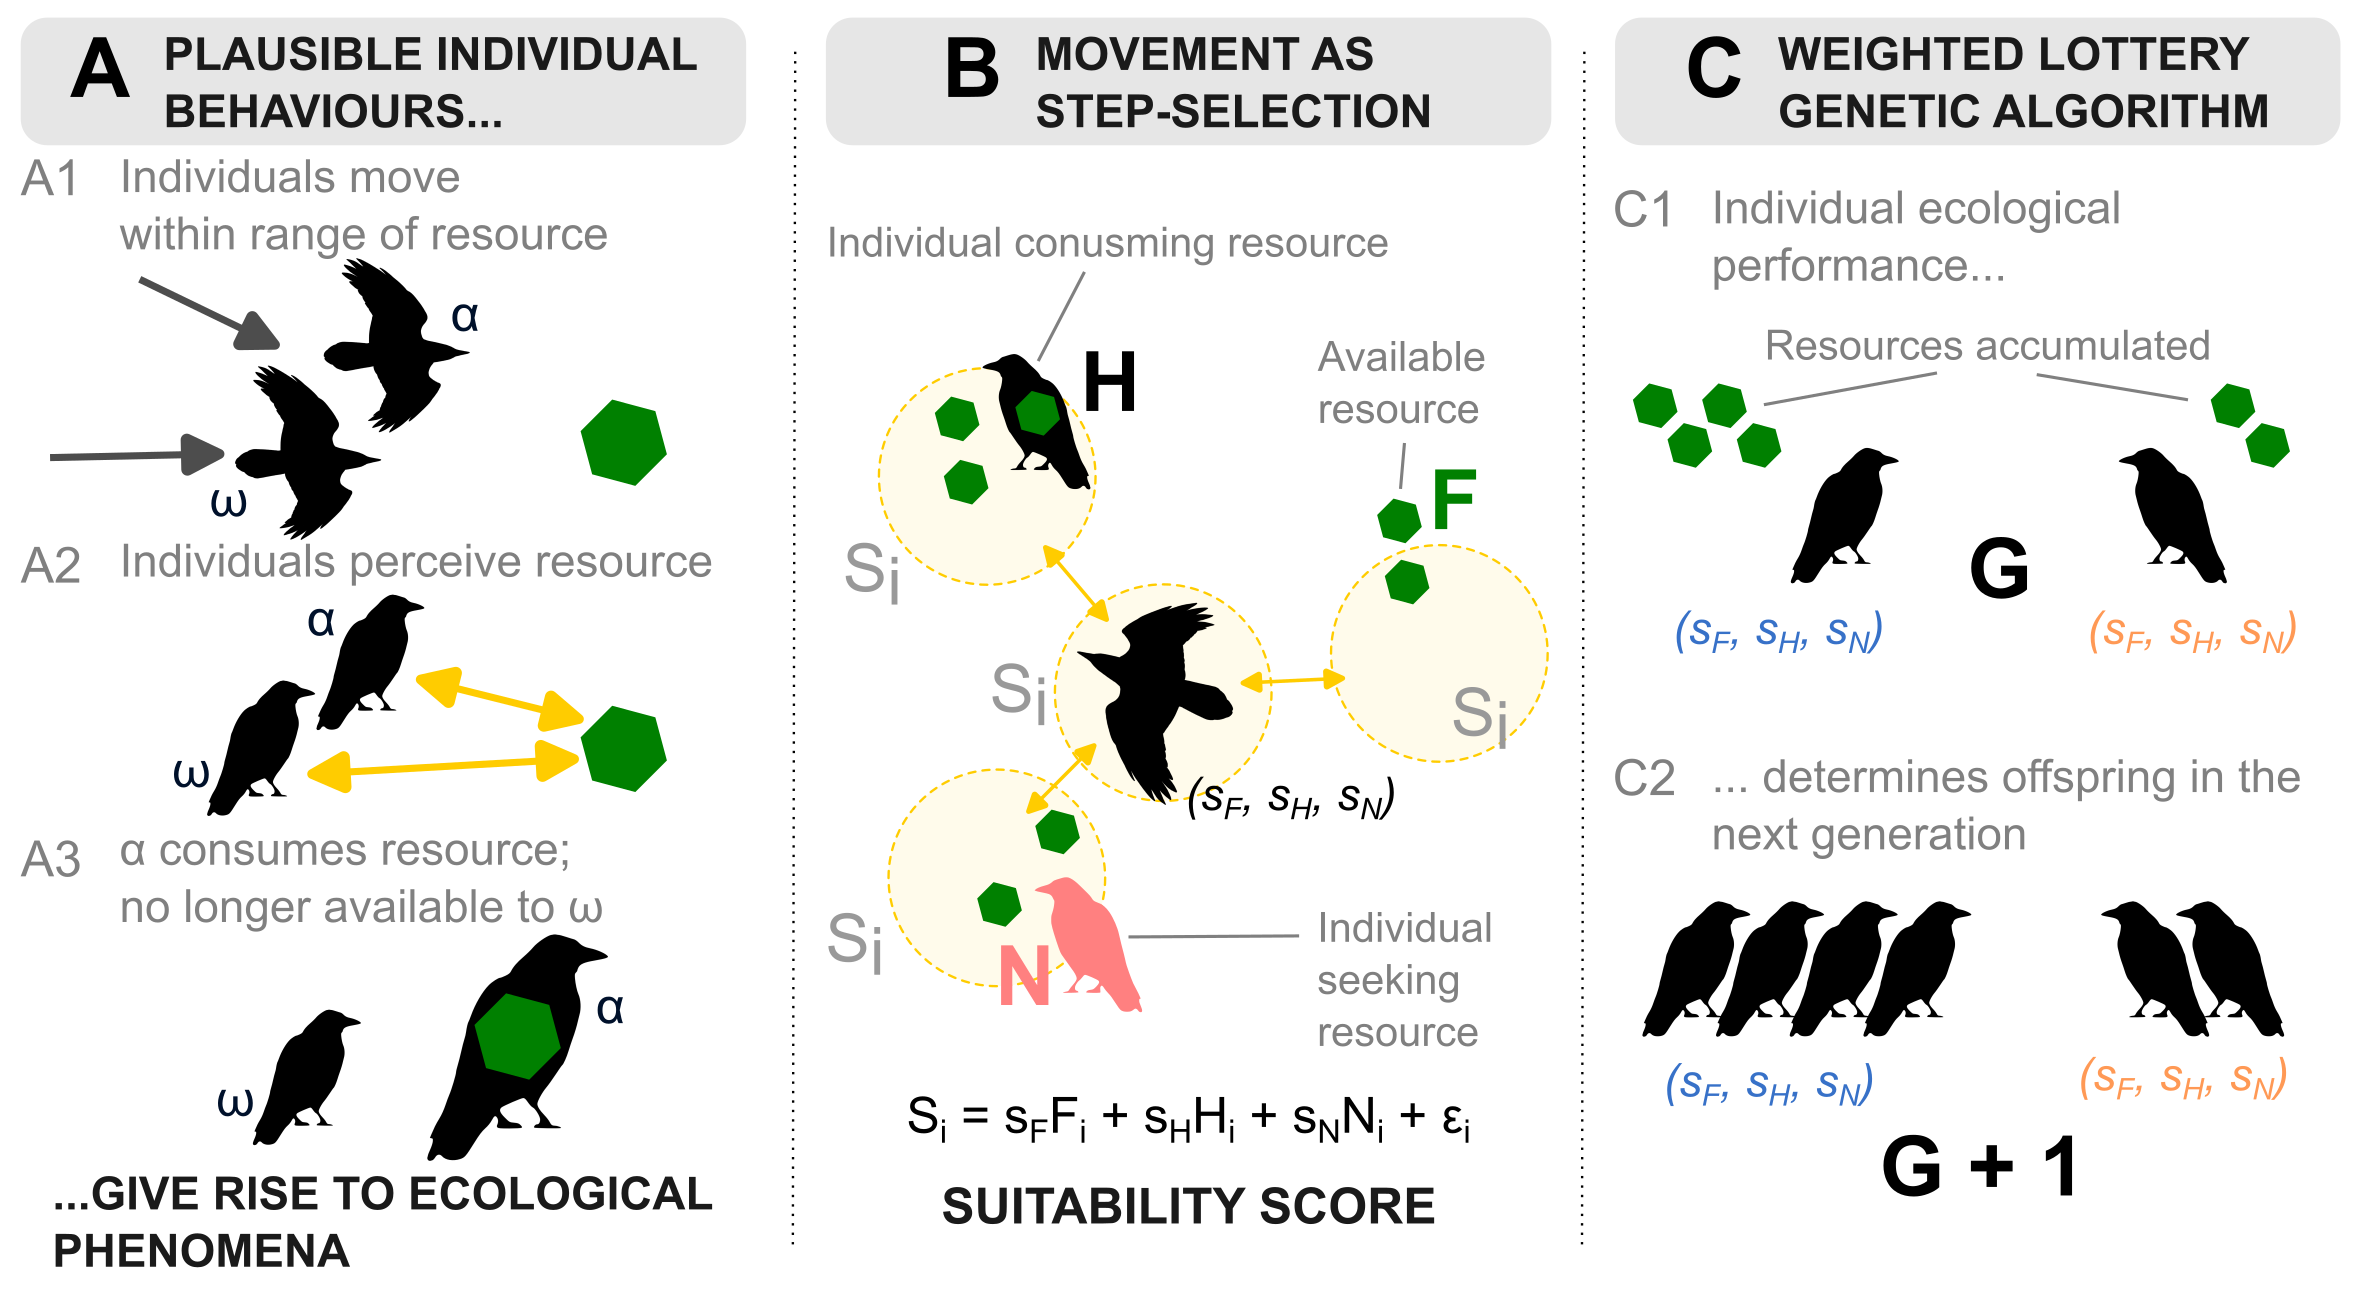
\includegraphics[width=0.9\linewidth]{figures/introduction/fig_concept.png}
  \caption{
      \textbf{Key conceptual ingredients of a mechanistic, individual-centric model of the eco-evolutionary dynamics of animal movement strategies.}
      \textbf{(A)} The model is individual-centric, and begins from first principles; model processes represent plausible, well supported animal behaviours, from which recognisable ecological phenomena may arise. Here, individuals' movement, perception, and consumption of resources leads to \textit{exploitation competition}.
      \textbf{(B)} Animal movement is modelled as sequential step-selection. Individuals perceive local cues, and assign `suitability scores' to potential destinations. Suitability at each location is calculated as the sum of the products of local cues (e.g. $F, H, N$) and the individual's cue preferences (e.g. $s_F, s_H, s_N$), with the optional addition of some small error in perception ($\epsilon$). Individuals move to the location with the highest suitability, which may be their current location (thereby remaining stationary). Both the cue preferences and cue values, and thus the suitability scores, can take any positive or negative values. It is the value of the cue preferences \textit{relative} to the other preferences, that determines the individual's \textit{movement strategy}.
      \textbf{(C)} The model integrates both ecological and evolutionary timescales, by allowing the ecological outcomes of animal movement (here, resource intake), to have evolutionary consequences. In this example, the individual with more intake has more offspring. Individuals pass on their movement-determining cue preferences to offspring (with some rare mutations); thus individual movement strategies in one generation can determine the population-level mixture of movement strategies in the next generation, setting up a feedback loop between the ecology and evolution of animal movement.
      All individuals are conceptually represented by crows for convenience; crow silhouettes are copyright free images submitted to \textit{PhyloPic}; see phylopic.org.
  }
  \label{fig:intro_concepts}
\end{sidewaysfigure}

\subsection*{Mechanistic, Individual-Centric Simulations}

The movement ecology paradigm recognises that animal movement is an individual-level process that integrates available external and internal cues into movement decisions \parencite{nathan2008a,holyoak2008}.
Furthermore, the proliferation of animals' traits via reproduction --- including cognitive traits such as movement strategies --- is dependent on individuals' ecological performance, upon which natural selection acts \parencite{hofbauer1988}.
Consequently we advocate for simulation models that follow this individual-centric approach.
Unsurprisingly, individual-based simulation models (IBMs) are ideal for this task, as they can include substantial ecological detail, including representing internal states, and interactions among hundreds of individuals and their environment \parencite{huston1988,deangelis2005,deangelis2018,deangelis2019}.

While researchers may begin modelling with a phenomenon in mind, it is important to shift perspective to instead encode plausible, well supported individual-level processes (which we also call mechanisms) that could give rise to such phenomena.
All ecological processes, including competition \parencite{keddy2001}, signalling and signal perception \parencite{torney2011}, memory-based navigation \parencite{bracis2017,robira2021}, and transmission processes (e.g. learning, pathogen transfer; see \cite{cantor2021,romano2021}) have a strong spatial component.
Thus models that study these phenomena should ideally also incorporate movement, and have an explicit spatial context.

For example, a model of exploitation competition would begin with the process that causes it: the depletion of discrete resource items due to individual foraging, which makes the resource unavailable to others \parencite[][; see Fig.~\ref{fig:intro_concepts}A]{keddy2001}.
This involves deliberately encoding a sequence of individual-level behaviours: movement that enables accessing a resource, perception of available resources, harvesting of the resource, and most importantly, removal of the resource from the landscape (see also \cite{spiegel2017,gupte2021a,gupte2022c}).
Here, the perspective shift lies in seeing that individual-level processes (movement, perception, foraging) could lead to the emergence of phenomena (exploitation competition), when local conditions are met (multiple individuals in the same vicinity going after the same discrete resource items).

Of course, any biological mechanism is an emergent outcome of constituent sub-mechanisms, down to the molecular level; some abstraction is therefore necessary.
For simplicity, some ecological and evolutionary aspects will have to be set aside.
This is not to say that issues such as sexual reproduction and non-random mating (included in \cite{getz2016}), detailed disease dynamics (seen in \cite{white2018,scherer2020}), flexible population sizes (as in \cite{netz2021}), or animal memory \parencite[e.g.][]{bracis2017,robira2021} are not important, but rather that researchers should focus on features of biological systems that are important to their study.
Classical analytical models regularly make similar modelling choices to arrive at conceptual insight (see an examination in \cite{vandermeer1997}).
Implementing these choices explicitly in simulation models' code helps bring these assumptions to the fore, promoting robust discussion of their importance to model conclusions.

\subsection*{Movement Strategies as Step-selection}

We conceive of individual movement across the landscape to take the form of sequential step-selection (which we call `movement decisions'; see Fig.~\ref{fig:intro_concepts}B).
Box A provides a primer to the idea of step-selection.
In our models, when the individual moves, it chooses among a number of potential destinations in its neighbourhood, including its current location (in which case it remains stationary).
Box B provides a brief overview of how step-selection has been used to encode movement in conceptual models.
The step choice is made by assigning each potential step (including the current location) a step-selection score, which we call the `suitability', such that every step $i$ has a suitability $S = s_{1}X_{1i} + s_{2}X_{2i} + \ldots + s_{N}X_{Ni} + \epsilon_i$.
Here, $s_n$ where $n \in (1, 2, \ldots N)$ is the individual-specific weight or `cue preference' for the cue $n$, and $X_n$ is the value of the cue at the location $i$.
We optionally include the small error term $\epsilon_i$ (typically drawn from a statistical distribution) to approximate individuals' error in assessing a location's suitability.
The cue preferences, and thus the suitability, can have arbitrarily large or small (positive or negative) values.
This is similar to step- and resource-selection coefficients $\beta$ \parencite[see Box A][]{fortin2005,manly2002}.
Individuals are considered to move to the location with the highest suitability.

\medskip

\begin{tcolorbox}[width=\textwidth,
    boxsep=0pt,
    left=0pt,
    right=0pt,
    top=2pt,
    arc=0pt,
    boxrule=0.0pt,
    toprule=1pt,
    bottomrule=1pt,
    colback=white
    ]%%
    \begin{description}[font=\scshape\bfseries]
        \item[Box A. Step-selection Analysis: An Introduction] Step-selection analysis is a method developed from the study of empirical animal movement data, which seeks to determine the drivers of animal movement, with an early implementation in \textcite{fortin2005}'s study of the movement of deer in response to wolves, in Yellowstone National Park.
        In brief, step-selection analysis contrasts locations at which animals were observed, against locations that they could have used instead \parencite[][]{fortin2005}.
        The locations that are considered to have been available to an animal are conditioned upon its current location --- essentially, this avoids comparing used locations with distant regions that the animal could not have used at that time.
        In this sense step-selection analysis is essentially similar to conditional resource-selection analysis \parencite[see as general reference][]{manly2007}.
        The difference is that in step-selection analysis, the available locations are sampled from a distribution (usually the Gamma distribution) fitted to the movement distances obtained from the tracking data, with relative headings (`turning angles'; see \cite{calenge2009}) drawn from a Von Mises distribution fitted to the animal's turning angles, again as seen in the tracking data \parencite[][]{thurfjell2014,signer2019}.
        The parameters determining the relative probability that a location is selected given its environmental attributes (the relative selection strengths, often denoted $\beta$) can be estimated via a maximum likelihood approach using common statistical software \parencite[see e.g. for R][]{therneau2000}.
        Overall, the step-selection method assumes that the probability that an animal will select a location is given by
        $$
            \hat{w}(x) = \text{exp}(\beta_1x_1 + \beta_2x_2 + \ldots \beta_nx_n)
        $$
        where $\hat{w}(x)$ is the selection score for a step, $\beta_i$ is the relative selection strength for (or against, if a negative value) the location attribute $x_i$.
    \end{description}
\end{tcolorbox}

\medskip

Crucially, when individuals move by step-selection as in our models, the value of each cue preference $s_{n}$ \textit{relative} to the other cue preferences is more important than the absolute value of any cue preference by itself (see also the `behavioural hypervolume' of \cite{bastille-rousseau2019}).
Thus individuals making movement decisions based upon three cues $X_n$ for $n \in (1, 2, 3)$, that have relatively similar values of the corresponding cue preferences $s_n$ may be thought of as weighing, or preferring each cue relatively equally (or indeed avoiding, if any $s_n < 0$).
The relative values of each individual's cue preferences \textit{taken together}, may be thought of as the individual \textit{movement strategy}.
Interlude~\ref{box:demos} shows how these strategies can be visualised and interpreted when they are comprised of a small number of preferences.

In our models, we assume individuals have a constant instantaneous speed, which means that all steps have the same distance \parencite[see a similar implementation in][]{spiegel2017}.
This is different from step-selection analysis of empirical data, which draws steps from a movement kernel \parencite{fortin2005,manly2002,avgar2016}.
Drawing steps from a kernel \parencite*[see e.g.][]{white2018} is \textit{not} mechanistic, as the movement kernel idea derives from a phenomenological description of movements observed from animal tracking or relocation data \parencite{fortin2005}.
Instead, our models allow movement kernels (and overall speeds, and `home ranges') to emerge from individual movement decisions (yet see below for an alternative).
Cues take the form of numeric values assigned to basic components of the individual's local environment, such the number of food items or of conspecifics (both integer values), or some environmental property, such as temperature (which could be a decimal value).
This allows individuals' movement decisions to be interactions of intrinsic, heritable preferences, and different components of the environment.
Spatio-temporal variation in cues can be externally forced (e.g. periodic fluctuations representing seasonality), but the much more interesting case is when such variation emerges from the movements and other behaviours of individuals.

There are two main mechanistic alternatives to our linear-function step-selection approach.
First, suitability scores could be computed using more complex functions (e.g. quadratic functions to allow for avoidance thresholds; see \cite{white2018}) --- but this could make movement strategies more challenging to understand.
Second, the movement process could be based on separately generating a movement distance and relative heading (`turning angle'; \cite{calenge2009}), rather than selecting from among steps \parencite{mueller2011}.
In contrast with our approach where individuals have a fixed speed, the latter approach allows variable speeds.
The drawback is that while movement distances are easily represented by linear functions, the turning angle is a circular measure that cannot be properly linearised.
A complex function such as an artificial neural network (ANN) --- standing in for an animal's cognitive mechanisms --- could generate both distances and valid turning angles, but the ANN parameters would be challenging to interpret as a movement strategy (\cite{mueller2011}; but see \cite{bastille-rousseau2019} for dimension reduction approaches).
Nonetheless, this approach is the preferable mechanistic alternative to assuming a movement kernel, as it too allows phenomenological movement descriptors (e.g. home range, step-length distribution) to emerge from individual movement decisions.

\afterpage{
    \medskip

    \begin{tcolorbox}[width=\textwidth,
        boxsep=0pt,
        left=0pt,
        right=0pt,
        top=2pt,
        arc=0pt,
        boxrule=0.0pt,toprule=1pt,
        bottomrule=1pt,
        colback=white
        ]%%
        \begin{description}[font=\scshape\bfseries]
            \item[Box B. Using Step-selection in Conceptual Models] Step-selection analysis is now widely used in animal movement ecology, with specialised implementations for habitat-specific movement characteristics \parencite{avgar2016}, decision points identified from very high-resolution data \parencite{munden2021}; it can also be extended to estimate animals' utilisation distributions \parencite{signer2017}.
            Indeed, recall that step-selection analysis is used even in this thesis (Chapter~\ref{ch:holeybirds}).
            Despite its popularity and ease of implementation, step-selection has seldom been used in individual-based simulation models of animal movement.
            One good example of using a step selection approach is \textcite{white2018}, who implemented a movement-disease model wherein individuals move across a grid, with their steps determined by their relative selection strengths ($\beta_i$) for cell attributes ($x_i$) such as resource levels or conspecific densities (in this sense they describe it as resource selection).
            In such models, individuals assign a selection score ($\hat{w}(x)$) to their current locations, and to neighbouring locations, and make the step with the highest score --- this may mean staying in place!
            Furthermore, $\beta_i$ values can be programmed to vary randomly or systematically in the population, to examine the effect of having individuals with a broad range of responses to similar cues (as \cite{white2018} do).
            In conceptual individual-based models such as mine, I refer to the selection score as `suitability'
            $
                S = \Sigma~s_{i}x_{i}
            $
            where $S$, the suitability of the potential location, is simply the sum of the interaction of the individual's selection strengths (which I call a `preference'; $s_i$) and the value of the corresponding cue at that location ($x_i$).
            In contrast with the step-selection approach, I assume that the individual moves in the direction of \emph{maximal} suitability. 
            Given that the `cue preferences' are individual properties, they can be considered to be heritable between generations of a population, allowing the examination of evolutionary dynamics.
            This concept is examined further in the final scenario of my model, and models implementing this approach are described in Chapters~\ref{ch:kleptomove} and \ref{ch:pathomove}.
        \end{description}
    \end{tcolorbox}

    \medskip
}

\subsection*{Integrating Ecological and Evolutionary Timescales}

The final feature of our model is the integration of ecological and evolutionary timescales.
This can be done by adopting the mechanistic, individual-centric approach and modelling reproduction; this allows individuals to pass on heritable traits --- including movement strategies --- to their offspring.
If individuals with better ecological performance are considered to have more offspring, this would lead to the proliferation of their strategies.
This would allow the mechanistic movement strategies to have evolutionary consequences, and in a scenario with discrete, non-overlapping generations, the ecological outcomes of individuals in one generation would determine the population-level mixture of behavioural strategies in the next generation.
The same evolutionary dynamics could be applied to individual traits other than the cue preferences as well, to potentially examine the co-evolution of movement with behavioural or physiological traits (see e.g. Chapter~\ref{ch:kleptomove}).
This approach, which we call the `weighted lottery', derives from population genetics, and specifically from the replicator equation, which is fundamental to evolutionary biology \parencite{hofbauer1988}.
The replicator equation states that the expected frequency of a strategy in the next generation is proportional to its frequency in the present generation, times the average lifetime reproductive success of individuals using that strategy.

% is essentially the `roulette wheel selection' approach of `genetic algorithms' (GAs) borrowed from computer science and artificial intelligence \parencite[although GAs were themselves obviously inspired by biology][]{sumida1990,hamblin2013,correia2010,deangelis2019}.

Here it is important to acknowledge that attempts to mimic biological evolution in individual-based models have previously been made, in the form of so-called `genetic algorithms' \parencite[GAs:][]{hamblin2013}.
Genetic algorithms have been applied to animal ecology, often coupled with individual-based models, but are relatively rare (see \cite{hamblin2013,beauchamp2007,hamblin2010,getz2015,getz2016}), possibly because their development and use is recognised as unsuitable for evolutionary biology.
While GAs were conceptualised to find the best solutions to complex optimisation problems, many eco-evolutionary contexts have no single, stable solution; moreover, environmental heterogeneity may mean that multiple solutions are equally viable \parencite{wolf2012}.
Furthermore, the GA conception of selection is often biologically unrealistic (e.g. truncation and tournament selection; \cite{hamblin2013}).
This is illustrated by \textcite{getz2015}, which uses a specific form of truncation selection, called `simulated annealing', wherein only the top 50\% of individuals reproduce, and the frequency of variation (essentially, the rate of mutations) becomes smaller with each generation --- neither of these are good representations of biological systems.
Consequently, I do not believe that the GA approach is broadly suitable for models that seek to study relatively open-ended evolution (although some specific cases may be useful; see `roulette wheel selection' in \cite{hamblin2013}).

% An important consideration when mimicking evolution is the introduction of variation.
% Studies using GAs take a wide range of approaches, but we advocate the independent \textit{per locus} method, in which each of the cue preferences has a probability of undergoing mutation.
% While GAs often draw the value by which a locus changes (the mutation size) from a normal distribution, we suggest that the Cauchy distribution is more appropriate; most mutations are small, but large, potentially consequential mutations could rarely occur.
% Further details of the evolutionary process, such as the mutation probability, or initial variation in cue preferences and traits in the simulation, can be varied based on study requirements.
% For instance, simulations with smaller populations ($<$ 1,000 individuals) could benefit from higher mutation rates to keep simulation run times low.

\section*{Versatility of Individual-Based Eco-evolutionary Models}

I focus on three broad yet relatively distinct classes of scenarios that are amenable to investigation using our mechanistic, eco-evolutionary modelling approach.
These are typically scenarios in which our current understanding of animal ecology suggests that multiple alternative or co-existing adaptive responses are possible.
I stress that this is how such models should be considered: as tools that enable the broad exploration of hypothetical scenarios, some of which I lay out below.
I caution against expecting eco-evolutionary dynamics known from analytical models; for instance, while steady-state eco-evolutionary equilibria may emerge in some models \parencite[e.g.][]{gupte2021a,gupte2022c,getz2015,getz2016}, it is unrealistic to expect such dynamics from all models \parencite[see e.g.][]{netz2021}.
Morever, an exploration of the parameter space, especially in terms of the environmental regime (e.g. environmental productivity, periodicity, or variation), could help generate broad predictive frameworks, with which empirical data could be compared.
Finally, as an added feature, I suggest how eco-evolutionary IBMs can be used to investigate the performance of statistical methods commonly used in animal ecology.

\subsection*{Changes in the Environmental Regime}

A key concern currently is knowing how the climate crisis is likely to affect animal spatial ecology, and I argue it is also important to know whether animal populations' evolutionary dynamics are likely to play a large role \parencite[e.g.][]{botero2015}.
For example, climate change is likely to induce greater variability in environmental conditions, thereby altering the spatial structure of resource landscapes (e.g. a transition from patchy to homogeneous resource landscapes).
When resources are more homogenously distributed, direct resource cues ($F$ in Fig.~\ref{fig:intro_concepts}) are likely to be more widespread, potentially reducing the importance of social information (conspecific presence; $H, N$ in Fig.~\ref{fig:intro_concepts}), which could indicate a resource cluster.
Yet with resources sparsely distributed, it may be important for animals to avoid conspecifics already at a resource cluster, to avoid exploitation competition --- this would require social information to acquire a high (negative) weight for movement decisions.
This scenario could be studied by building a model wherein the landscape spatial structure is altered after an initial (long) period of stability.
Key questions that could be answered with such models are include whether a change in resource spatial structure --- without a change in actual abundance --- can lead to changes in movement strategies; whether movement strategies evolved to deal with changed spatial structure then also result in a non-ideal distributions of animals relative to resources \parencite[a test of][]{fretwell1970,parker1978}; and whether different animal social structures could emerge \parencite[see][]{webber2022,tanner2012}.

\subsection*{Joint Evolution of Movement and Behavioural Strategies}

Animal movement strategies alone are insufficient to explain individuals' ecological niches; individuals must combine these with other decisions, such as which resources to exploit \parencite{vangils2015,pulliam1974}.
In a scenario where there are two distinct types of prey, individuals could potentially prefer to use the locally more abundant prey \parencite{emlen1966,pulliam1974}.
Alternatively, individuals could specialise upon one of the two prey types; this could be on the prey type preferred by most other individuals (whereby social information on prey clustering could be useful; positive density dependence), or indeed upon the less preferred prey type, as this could reduce competition (negative density dependence).
In this context, it is not clear how prey type preferences would evolve, but movement and foraging strategies could potentially be correlated, making it an ideal case for exploration with the class of models I advocate.
This scenario could be explored with a model containing two overlapping prey type distributions, say $A$ and $B$, and allowing individuals to sense and have a preference for these different prey types ($s_A, s_B$, instead of $s_F$ in our Fig.~\ref{fig:intro_concepts}).
Simultaneously, it would be appropriate to consider prey choice to also be a flexible decision, and allow individuals to mechanistically choose, at each step, which prey type they want to target.
% This entails introducing four more intrinsic, individual-specific `behavioural preferences': $w_A, w_B$, for the prey counts $A, B$, and $w_H, w_N$, for the handler and non-handler counts $H, N$.
% Together with local cues, they could be combined into a prey type choice, where $W = w_AA + w_BB + w_HH + w_NN + \epsilon$, where the individual chooses prey $A$ if $W < 0$, and $B$ otherwise (the simplest binarisation of a continuous response).
Such a simulation could reveal the emergence of substantial individual variation in the preferences for the prey types, and potentially correlations with foraging movement strategies, forming a movement-behaviour syndrome (see e.g. \cite{eckhardt1979}).
More specific prey choice models could investigate how foraging individuals themselves may be a type of prey, through kleptoparasitism --- this scenario is explored in Chapter~\ref{ch:kleptomove}.
Models could also be extended to multiple trophic levels by including predators, in order to study the evolutionary arms-race of movement strategies between predators and prey \parencite{netz2021}.

\subsection*{Introduction of New Eco-evolutionary Dynamics}

The introduction to an environment of a novel biotic component could substantially alter existing eco-evolutionary dynamics; the introduction of a novel pathogen (or strain) to a population is a key example of current relevance (\cite{carlson2022a}; see also \cite{monk2022} as a case study).
Novel pathogen introductions should be expected to impose selection against animal sociality \parencite[e.g.][]{ashby2022}, but sociality emerges from an interaction of individual behaviour and the local environment, including the social environment \parencite{tanner2012}.
To examine how a novel pathogen could affect the evolution of animal movement strategies, our modelling framework could be adapted into a movement-disease model following templates in \textcite{white2018a}.
% modified such that, after adapting to their landscape for a few thousand generations, a small percentage ($<$ 5\%) of individuals in each generation are considered `infected' in each following generation by a novel pathogen, possibly spread to them by some other overlapping species (e.g. as in \cite{monk2022}).
For instance, a pathogen could spread among spatially proximate individuals with some small probability $p$, and impose an energetic (and hence, fitness) cost $\delta E$.
Such a model could reveal whether the novel pathogen introductions impose selective pressure against individual preferences for sociability as a proxy of transmission risk \parencite{weinstein2018}.
Such a scenario, with special reference to social information use, is explored in Chapter~\ref{ch:pathomove}.
Recording and logging spatial associations and pathogen transmissions among simulation individuals could help provide useful expectations against which to compare transmission dynamics inferred from animal tracking data (\cite{wilber2022}; see \cite{robitaille2019,albery2021} for background).

\subsection*{Using Mechanistic Models to Probe Current Statistical Methods}

Movement models are regularly used to simulate tracks with known features in order to examine and improve the performance of statistical tools \parencite[such as segmentation algorithms; see e.g.][]{gurarie2016,michelot2016,patin2020a}.
One area which could benefit from a similar understanding of commonly used methods is the study of individual variation in movement; specifically, this could help determine whether studies are truly picking up `spatial personalities' from the confounding factors of environmental differences among tracked animals \parencite{stuber2022,spiegel2022}.
% Animal movement researchers apply sophisticated variance-partitioning approaches to movement data to estimate how much behavioural variation in a population is explained by individual identity \parencite[especially using `repeatability analysis'][]{hertel2020, hertel2019, hertel2021,nakagawa2010}.
% Simultaneously, step- and resource-selection functions coefficients estimated from animal tracking data can also be analysed in order to detect distinct behavioural clusters \parencite{bastille-rousseau2019}.

The class of mechanistic movement models I advocate could help explore whether current statistical tools can reliably detect individual differences in movement decision-making mechanisms.
For instance, recording the movement paths of model agents, as well as their cue preferences and other traits (e.g. evolved prey-type preferences), and applying a repeatability approach, could help determine how the fitting of certain individual attributes as fixed effects could affect repeatability scores (\emph{vs.} leaving them out).
Similarly, recording the local cues available to individuals while making movement decisions would yield exactly the matched case-control data used in fitting step-selection functions \parencite[see][]{signer2019}
Sub-sampling this data (to simulate low-resolution tracking), or using a static predictor such as landscape productivity (as is often used in empirical studies; e.g. NDVI: \cite{pettorelli2011}) could help demonstrate the benefits of using high-throughput tracking \parencite{nathan2022}, and the issues around using broad static predictors of landscape conditions.
Overall, by treating a simulation model with simple movement strategies as one would empirical animal tracking data, one could explore the performance of popular statistical tools with data from known eco-evolutionary contexts --- Chapter~\ref{ch:patternprocess} explores this scenario.

\section*{Structure of this Thesis}

In this Thesis, I take a broad approach to study both animal movement ecology, as well as presenting a framework for conceptual models to study the evolution of animal movement strategies. The thesis is divided into two parts, with five main chapter that are described here.

\medskip

Modern movement ecology has become a `big data' field \parencite{nathan2022}.
In Part~\ref{part:eco} I focus on studying animal movement ecology using tracking data and correlative statistical models, but from a strongly mechanistic perspective.
In Chapter~\ref{ch:preprocessing}, I synthesise methods that can help overcome current limitations and issues in modern high-throughput tracking data.
I present conceptual workflows to prepare high-throughput animal tracking data for further analysis, and may be seen as a more detailed explanation of the principles I contributed to \textcite{nathan2022}.
In brief, modern, high-throughput animal tracking increasingly yields `big data' at very fine temporal scales, and `cleaning' the data to reduce location errors is one of the main ways to deal with position uncertainty.
Though data cleaning is widely recommended, robust guidance on how to organise the cleaning of massive datasets is relatively scarce.
A pipeline for cleaning massive high-throughput datasets must balance ease of use and computationally efficiency, in which location errors are rejected while preserving valid animal movements. 
Another useful feature of a pre-processing pipeline is efficiently segmenting and clustering location data for statistical methods, while also being scalable to large datasets and robust to imperfect sampling.
One major advantage when studying a particular species is that certain aspects of its biology are known --- for example, the maximum speed it could realistically achieve.
These physical constraints can be taken into account to filter data, and identify behavioural bouts in ways that are easy to interpret \parencite[][]{barraquand2008}.
I show how taking this mechanistic view to filtering animal positioning data can be used with any high-throughput animal movement data in which the high data-volume combined with knowledge of the tracked individuals' biology can be used to reduce location errors.

In Chapter~\ref{ch:holeybirds}, I leverage the methods for improving and working with high-throughput tracking data that I developed in Chapter~\ref{ch:preprocessing}.
I take an explicitly mechanistic view to studying the drivers of movement and habitat selection in a unique group of animals: moulting birds.
The flight surfaces of bird wings require regular renewal through a process called moult --- shedding worn out feathers and growing fresh ones --- presenting birds with the dilemma of needing more resources for feather growth just when their flight capacity is reduced, making them more vulnerable to predation.
I combine animal tracking and experimental approaches to present a first quantification of the direct effects of wing moult (in terms of reduced flight efficiency) on the movement and use of sheltered habitats, in four non-migratory passerine species.
Rather than using a broad predictor such as vegetation productivity as a proxy for shelter \parencite{pettorelli2011}, I instead take a viewshed ecology approach \parencite{aben2018}, and directly quantified which areas of the landscape were visibile to potential predators \parencite[the `fearscape':][]{olsoy2015}.
I use the methods, including the residence patch algorithm, developed in Chapter~\ref{ch:preprocessing}, to measure how non-moulting, naturally moulting, and artificially manipulated birds use sheltered areas.
I apply both simple statistical models as well as step-selection analyses to analyse birds' habitat selection \parencite{fortin2005,avgar2016}.
Later, in Part~\ref{part:evo}, I use the models described there to examine what we can learn about step-selection analysis, by using it to recover the mechanisms of simulation models (a better explanation of the links between the two is presented in Chapters~\ref{ch:kleptomove}).

\medskip

In Part~\ref{part:evo}, I demonstrate how conceptual insights can be obtained from mechanistic models of intermediate complexity that integrate both the ecological dynamics of animal movement, and their evolutionary causes and consequences.
The key feature of such models is to let individual-level ecological outcomes in one generation influence which movement strategies are present in future generations, thus establishing a feedback loop between animals' evolutionary history and their current spatial ecology.
Specifically, I advocate that movement be modelled as an individual response to local cues rather than a random walk or some ruleset shared by all individuals \citep[see][]{mueller2011}.
I have taken this mechanistic in Chapters~\ref{ch:kleptomove} and \ref{ch:pathomove}.
In the models presented in those chapters, I used individual-based models, in which individuals have evolved \emph{movement preferences} --- these are explained below --- and thus make quite different decisions when presented with similar cues \citep{getz2015,white2018}.
Yet an open question when including such behavioural variation is whether the emergent outcomes may be transient phenomena that are quite different from the dynamics obtained on evolutionary timescales.
% This is especially the case when modelling processes that have fitness consequences for some behavioural types (such as disease in \cite[]{white2018}).
Consequently, I additionally advocate for movement models to be embedded in an evolutionary context, with individuals' movement outcomes subject to selection, and their movement preferences subject to random change (mutation).
I expand on this view further in this Introduction, and describe the three chapters comprising this Part in brief below.

In Chapter~\ref{ch:kleptomove}, I examine the joint evolution of movement and two different foraging strategies: searching for food items, and kleptoparasitism, an extreme form of interference competition.
Although competition has an explicit spatial context, eco-evolutionary models rarely consider how competition strategies, including kleptoparasitism, might evolve alongside evolving movement strategies.
I model movement strategies as heritable, individual-specific combinations of preferences for environmental cues, similar to step-selection coefficients \parencite{fortin2005,manly2002}.
Step-selection coefficients have been used previously to cluster individuals with different preferences for local cues into discrete strategies \parencite{bastille-rousseau2019}.
I study the evolutionary dynamics of competition and movement strategies using individual-based simulations.
I additionally, investigate the implications of this joint evolution for the distribution of consumers over the model landscape.
Overall, this chapter lays the groundwork for a mechanistic approach to studying competition --- and other behaviours --- in a spatial context, and suggests how evolutionary modelling can be integrated with current work in animal movement ecology.

In Chapter~\ref{ch:pathomove}, I aim to investigate a scenario that pre-occupied me over the course of the pandemic: the evolutionary consequences of the introduction of novel pathogens for animal social interactions, which are of course, outcomes of animal movement.
Using a simulation model developed from the work I presented in Chapter~\ref{ch:kleptomove}, I examine how animals balance the risk of pathogen transmission against the benefits of public information about the location of ephemeral resource patches.
Studying a scenario in which a fitness-reducing infectious pathogen is introduced into a population which has initially evolved movement strategies in its absence, I show how pathogen introduction changes host movement strategies, and how this determines the emergent structure of socio-spatial networks.
The use of the deterministic step-selection framework borrowed from Chapter~\ref{ch:kleptomove}, which can be directly related to step-selection analyses conducted on empirical animal tracking data \parencite{bastille-rousseau2019}, makes this a powerful modelling framework, with initial predictions for the evolutionary and ecological consequences of wildlife pathogen spillover scenarios.

In Chapter~\ref{ch:patternprocess}, I apply two popular statistical methods, repeatability analysis, and step-selection analysis, to the movement paths generated by agents from Chapter~\ref{ch:kleptomove}.
Having encoded these agents to move using simplified step-selection, here, I examine what current statistical methods in movement ecology can tell us about individual variation in a population where the axes of variation are already fully known.
I show how it is challenging, to recover the true causes of variation in animals' movement strategies from their actual movement paths (a major line of work in movement ecology).
I demonstrate that statistical methods can yield quite different conclusions when applied to data in which underlying movement strategies are not accounted for, and therefore caution practitioners analysing empirical data to be careful with potential sources of behavioural variation.

Finally, in Chapter~\ref{ch:discussion}, I reflect upon the findings of this thesis, and upon potential future work.

{ \begin{center} \barfont{-.-} \end{center} }

%%%%%%%%%%%%% Supplement %%%%%%%%%%%%%%%

\clearpage
